\section{Multi-container applications}
Over the years \gls{EPICS} has become a framework that offers users many off-the-shelf applications that ease the implementation and configuration of a control system. Figure \ref{fig_dcs_node_msts} shows the most commonly used control-related applications. 

All the applications in figure~\ref{fig_dcs_node_msts} applications were used as containers based on prepared images and linked using Docker-compose, which is a tool for defining and running multi-container Docker applications~\cite{docker_compose}. To configure the containers a YAML\footnote{YAML is a human-friendly data serialization language for all programming languages~\cite{YAML}.} file has to be populated with the services settings (in this case the services refer to the applications, e.g. \gls{IOC}. This section summarizes the most important applications used for the \gls{DCS} and their functionalities.


\begin{figure}[!h]
\centering
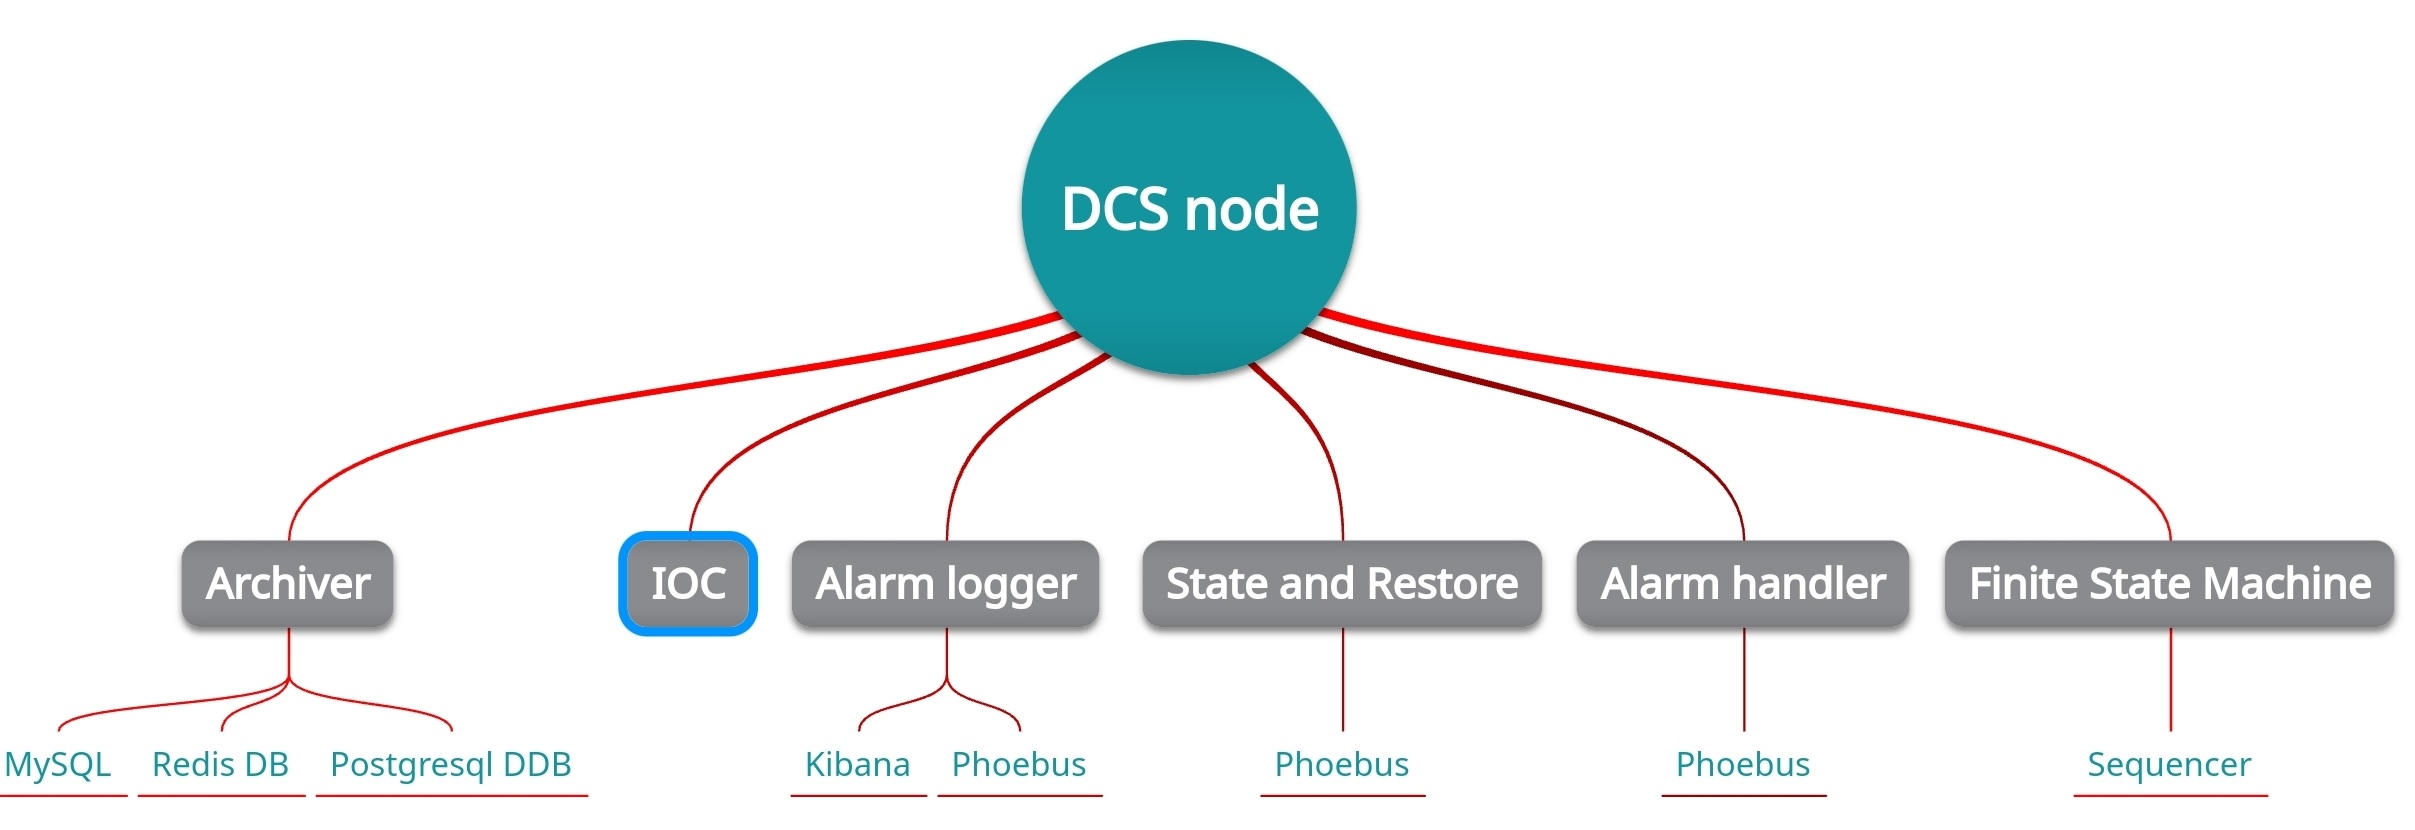
\includegraphics[width=0.95\columnwidth]{Chapter4/images/dcs_node.jpg}
\caption{Services used in addition to Phoebus functionalities, together forming a full-blown control system.}
\label{fig_dcs_node_msts}
\end{figure}
\newpage
\subsection{Control System Studio and Phoebus}

Control System Studio (\gls{CSS}) consists of open-source Java applications and modules which can be used in constructing a control system. Phoebus is an update to the \gls{CSS}, and significantly improves its performance by removing dependencies on Eclipse RCP. Phoebus uses both channel access protocol and \gls{PV} access, and it offers graphically based applications to access \gls{EPICS} \glspl{PV}, \glspl{OPI}, PVs history, etc. An example of a chiller \gls{GUI} is depicted in figure~\ref{fig_lauda1}. One of the main features of Phoebus is its modular nature. Users can develop and add their products, or just include or exclude applications or configurations. 


\begin{figure}[!h]
\centering
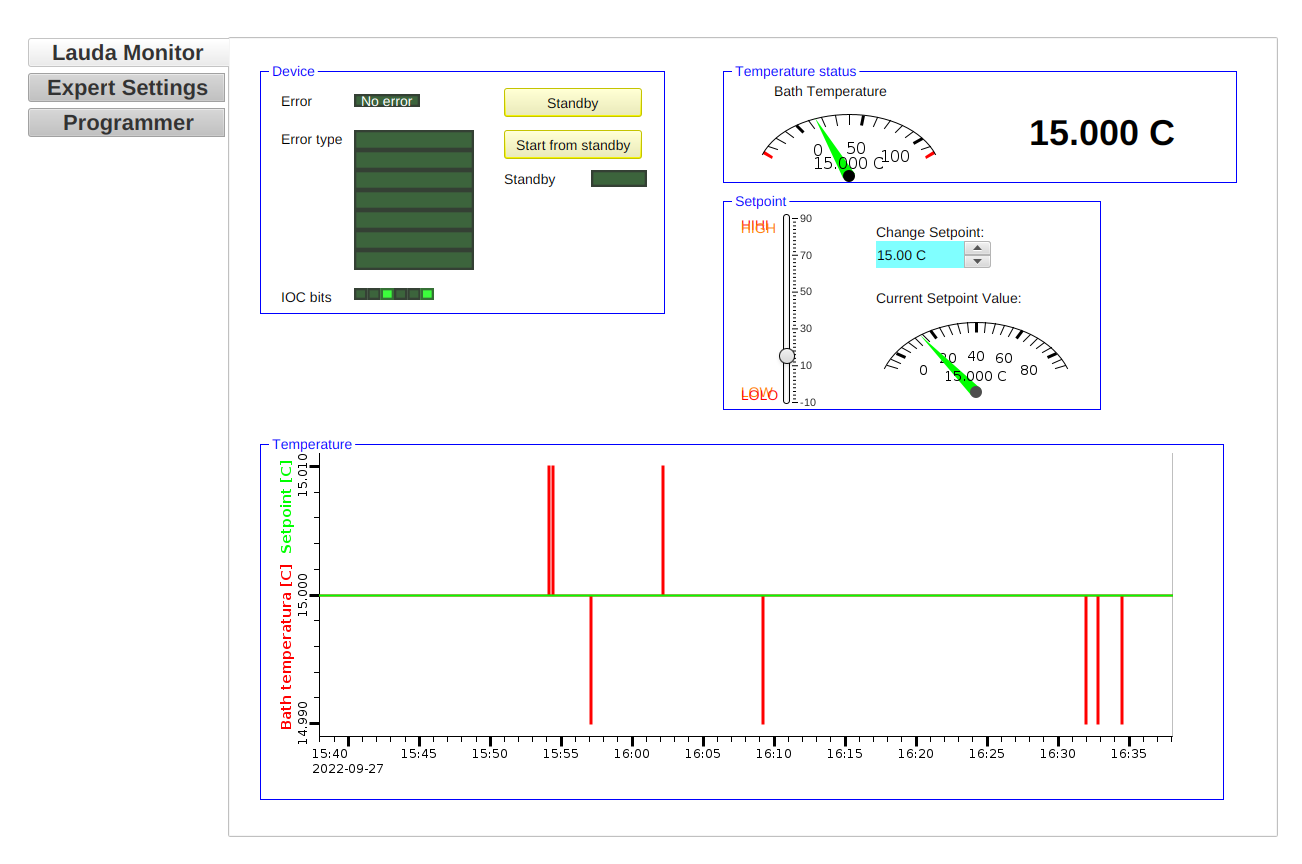
\includegraphics[width=1\columnwidth]{Chapter4/images/lauda1.png}
\caption{An example of a detector system \gls{GUI} for a cooling unit.}
\label{fig_lauda1}
\end{figure}

\newpage
\subsection{Solutions for archiving the data} \label{archiver}
An Archiver serves as one of the main building blocks of the \gls{DCS}, as it allows not only to look up the history of a given record, but also to download and post-process the data. Archivers make use of the publish/subscribe logic, updating the values on change. In general, the archiver must run smoothly, without significant downtime, and the linked database and other clients should also have a stable connection. A primary choice for \gls{STS} is the so-called Archiver Appliance~\cite{archiver_appliance}. An example of the archiver appliance is divided into short-term storage, medium-term storage, and long-term storage. In principle, a system administrator can adjust these settings to the needs of the specific case. The  four Tomcat containers\footnote{An Open source web server by the Apache foundation} are employed to handle the tasks of the archiver.  
%\begin{figure}[!h]
%\centering
%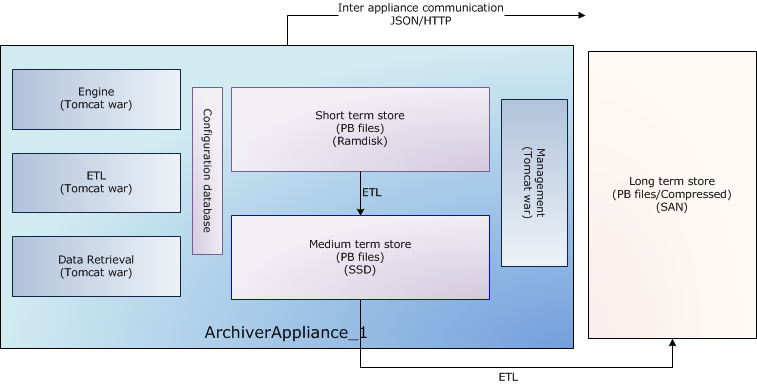
\includegraphics[width=0.7\columnwidth]{Chapter4/images/applarch.png}
%\caption{Architecture of a single appliance \cite{archiver_appliance}}
%\label{fig_archiver}
%\end{figure}
%\newline

The main advantage of the archiver include: 

\begin{itemize}
    \item Data retrieval can be integrated into Phoebus or Matlab,
    \item Wide range of supported formats,
    \item stable performance, even with a hundred thousand \glspl{PV}.
\end{itemize}

Apart from the Archiver appliance, there are also alternative solutions:

\begin{itemize}
    \item Cassandra \cite{cassandra_archive},
    \item RDB Archive engine \cite{rdb_archive}.
\end{itemize}

\subsection{Alert communication with alarm server}
An alarm server monitors a chosen set of \glspl{PV}, including their alarm state. \gls{EPICS} records facilitate fields related to the alarm thresholds and their severity, evaluated each time the record is processed. Every numeric value could have two uppers and two lower boundaries, with assigned severities (NO\_ALARM, MINOR, MAJOR). \gls{EPICS} by itself, doesn't take any actions on the detector's hardware when the alarm threshold is exceeded. On the other hand, a Phoebus-based \gls{GUI} will change the font color (MINOR - orange, MAJOR - red) of the variable once the alarm appears. If the connection to the alarm server exists, then the server acts upon a change in the alarm status of a record. The user interfaces show alarms, allow acknowledgment, and provide guidance and helpful links. Apache Kafka is a distributed event store and stream-processing platform which serves as a communication bus between the alarm server and Phoebus. An example of the \gls{mSTS}'s alarm handling \gls{GUI} is depicted in Figure~\ref{fig_alarm1}. It provides not only a visual notification of an alarm but also guidance, displays, and commands.
\begin{figure}[!h]
\centering
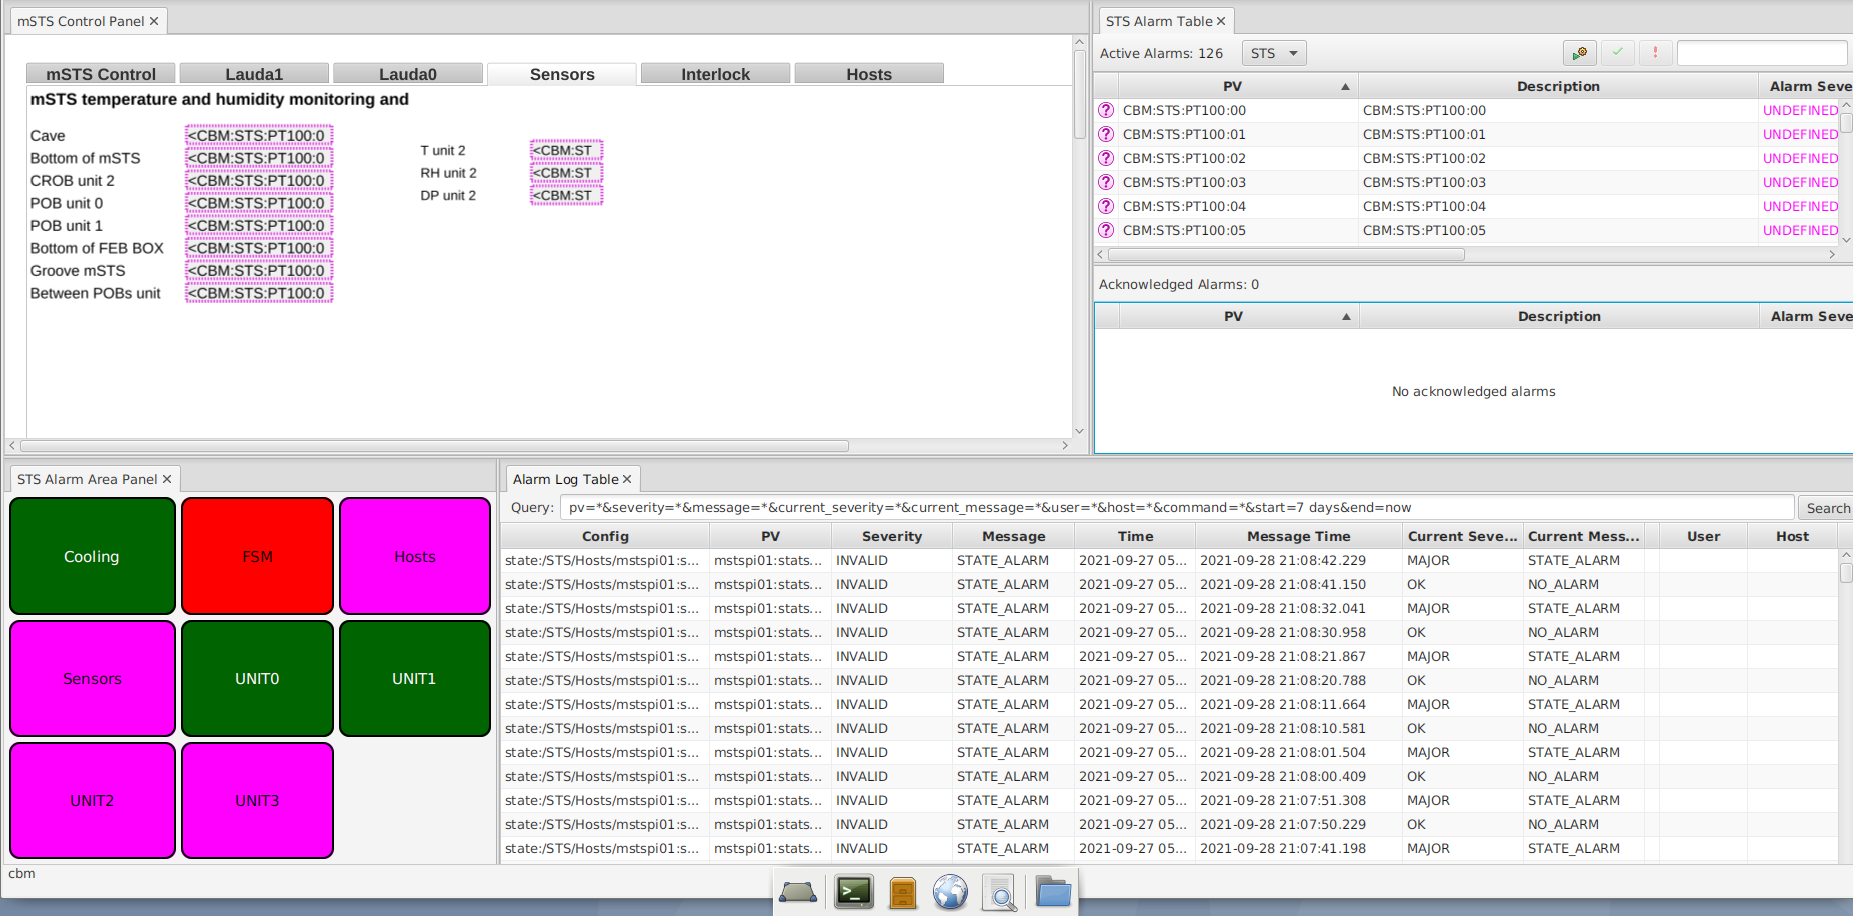
\includegraphics[width=1\columnwidth]{Chapter4/images/alarms.png}
\caption{Phoebus alarm handler view -  top left part some \gls{GUI}s, the top right part is the alarm table showing the current and acknowledged alarms, bottom left features a color status of respective nodes (e.g. cooling), bottom right shows the latest entries in the log.}
\label{fig_alarm1}
\end{figure}
\newpage
\subsection{State and commands logging}
Logging is another important part of the \gls{DCS}. It allows monitoring and checking of all the changes in the configuration and alarms of all the process variables. Thanks to the logs acquired by the dedicated service, debugging becomes much easier. The alarm logging service enables the logging of: configuration changes, state changes logging, and commands. Similarly to the alarm server, it uses Apache Kafka for data transfer. Apart from the logs, there is also a \gls{GUI} available in the Phoebus \cite{alarm_logger}, an operator can also use the Kibana\footnote{source-available data visualization software} web interface to discover patterns and trends in the data. 

\subsection{Finite state machine as an automation and safety mechanism}
A finite state machine (\gls{FSM}) is a construct that defines states and transitions between these states. In a given moment it has a clearly defined state and a given set of rules and conditions apply to this state. An input issued by an operator or automatically by a sensor(s) could trigger a transition. All transitions are unidirectional, but it's possible to define two opposite transitions, e.g. entering and escaping the error state. 
\newpage
One of the possibilities to implement a \gls{FSM} is to use Sequencer, which is a State Notation Language based on C/C++. 
\begin{itemize}
    \item start-up, shut-down, fault recovery, etc.,
    \item little C code, many states, many transitions,
    \item short compilation time, and can call any C++ code, easy connection to channelAccess.
\end{itemize}

One of the alternatives to the Sequencer and State Notation language is the PyEPICS-based library Pysmlib. It features several interesting functions like integrated watchdog logic, multi-threading, or configurable logging systems.


\section{Containerized EPICS-based framework}

The containers-based framework introduced in this chapter is the baseline for all the research and development activities throughout this thesis. In principle, most small and/or laboratory-based experimental setups don't require full-blown control systems. Hence, in the next two chapters two smaller framework applications will be introduced. In addition to that, the studies and their implications are discussed in detail. Chapter 6 is dedicated to the application of the full control system to the Phase-0 version of the \gls{STS}.